\section{Funktionsweise}
\label{sec:funktionsweise}
Prinzipiell dreht sich die App um zwei essentielle Funktionen. Die Registration und der Alarmempfang. Diese beiden Funktionalitäten werden nachfolgend genauer beschrieben.
\subsection{Registration}
\begin{figure}[htbp]
	\centering
	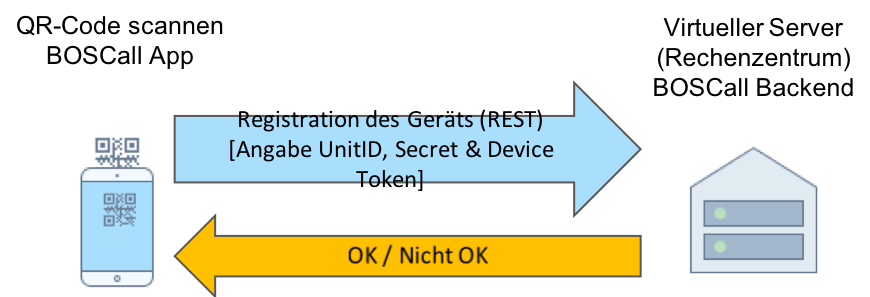
\includegraphics[width=\linewidth]{include/img/registration}
	\caption{Registration}
	\label{fig:registration}
\end{figure}
Anforderungen an die Registration war eine möglichst geringe Komplexität und zugleich eine hohe Sicherheit zu realisieren. Der Fokus lag aber zwecks des begrenzten Entwicklungszeitraums auf der geringen Komplexität.

Um die Komplexität zu reduzieren wird jedem Leiter einer Einheit ein QR-Code ausgestellt, der dazu dient, dass sich Mitglieder registrieren können. Es ist für den Anwender also nur erforderlich, dass er seinen Namen eingibt und einen QR-Code mit seiner Smartphone Kamera scannt. In diesem QR-Code befinden sich alle Details, die zur Registration erforderlich sind. Zum Beispiel die ID der Einheit (UnitID) und der private Schlüssel (Secret). Zusätzlich sendet das Gerät bei der Registrationsanfrage den eigenen Gerätetoken (Devicetoken) mit. Damit können Push Nachrichten gezielt an das Endgerät gesendet werden.

\subsection{Alarmempfang}
\begin{figure*}[htbp]
	\centering
	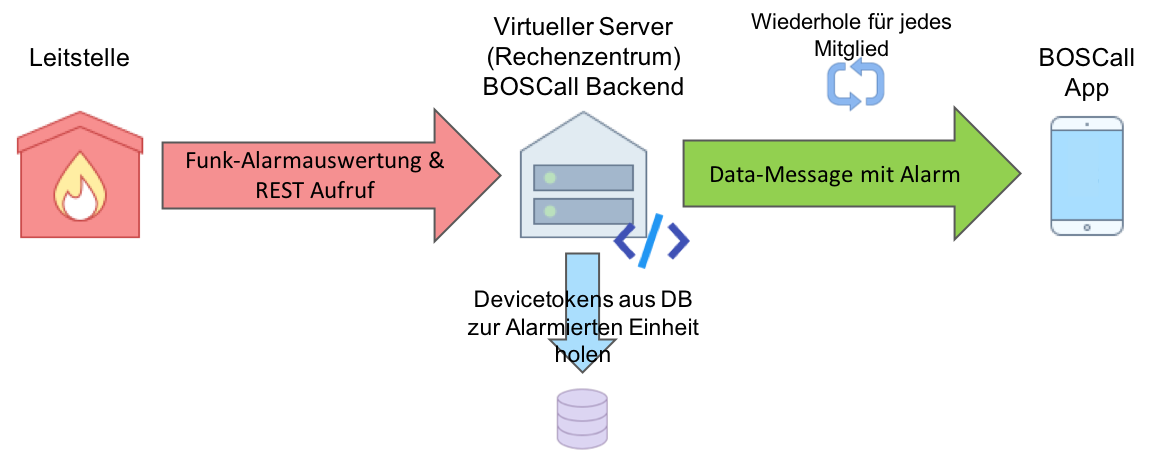
\includegraphics[width=\linewidth]{include/img/alarmablauf}
	\caption{Alarmablauf}
	\label{fig:alarmablauf}
\end{figure*}
Der Ablauf der Alarmierung, graphisch in Abbildung~\ref{fig:alarmablauf} zu sehen, teilt sich in drei Schritte. Zunächst wird der Alarm über eine Auswertung des analogen Funks erkannt und es wird die E-Mail der Leitstelle mit den Einsatzdetails ausgewertet. Dieser Prozess wird nicht durch die Anwendungen abgedeckt, die im Rahmen der Veranstaltung entwickelt wurden. Es gibt bereits eine funktionierende Bestandsanwendung, die sich relativ problemlos auf die Unterstützung von BOSCall ändern lässt.

Im nächsten Schritt wird durch die soeben genannte Anwendung per HTTP Aufruf (REST) ein Alarmprozess angestoßen. Der Dienst, der dabei aufgerufen wurde, liegt dabei auf einem öffentlichen virtuellen Server. Der Service wertet nun den eingegangenen Alarm aus indem er die Einheit aus der Anfrage bezieht. Mittels diesem Datum bekommt er aus einer Datenbank alle registrierten Endgeräte dieser Einheit. Deren Token nutzt er um über die API von Firebase eine Push Nachricht an das Gerät zu senden.

Im letzten Schritt wird die erhaltene Push Nachricht auf dem Endgerät ausgewertet. Diese sogenannte Data Message enthält alle Daten, die für die Darstellung einer Alarmierung benötigt werden, also Alarmtitel und Alarmtext. Es gilt hier zwischen Data Message und einer sogenannten Notification Message zu unterscheiden. Diese Unterscheidung bereitete zunächst Probleme, weshalb diese beiden Typen weiter im Kapitel~\ref{sec:problemstellungen} erläutert werden.